% ============================================================================
% CHƯƠNG 4: TRIỂN KHAI & ĐÁNH GIÁ
% ============================================================================
\chapter{TRIỂN KHAI \& ĐÁNH GIÁ}

Chương này trình bày kết quả triển khai hệ thống L-RAG và đánh giá định lượng chất lượng trên ba Phase: (1) Ingestion — so sánh LSU Chunking với Fixed-size Chunking, (2) Alignment — so sánh Hungarian Matching với Greedy Matching, và (3) Generative Comparison — đánh giá hiệu quả của cơ chế chống ảo giác 3 tầng.

% ============================================================================
\section{Môi trường Triển khai}
% ============================================================================

Hệ thống được triển khai trên cấu hình phần cứng như sau:

\begin{table}[H]
    \centering
    \caption{Cấu hình phần cứng triển khai}
    \label{tab:hardware}
    \begin{tabularx}{\textwidth}{l X X}
        \toprule
        \textbf{Thành phần} & \textbf{Thông số} & \textbf{Ghi chú}\\
        \midrule
        GPU & NVIDIA RTX 4090 (24GB VRAM) & Đủ cho BGE-M3 FP16 (2GB) + Qwen2.5-7B Q4\_K\_M (5GB)\\
        CPU & Intel Core i9 / AMD Ryzen 9 & Xử lý parsing và verification\\
        RAM & 32--64GB & Load model weights + xử lý batch\\
        OS & Ubuntu 22.04 LTS & \\
        Python & 3.10+ & \\
        \bottomrule
    \end{tabularx}
\end{table}

Tổng \gls{vram} usage khi chạy pipeline tuần tự: BGE-M3 (FP16) $\sim$2GB, Qwen2.5-7B (Q4\_K\_M GGUF) $\sim$5GB, KV Cache + overhead $\sim$1GB. \textbf{Tổng: $\sim$8GB} — rất thoải mái trên RTX 4090 (24GB). Pipeline chạy tuần tự: embed toàn bộ $\rightarrow$ align $\rightarrow$ rồi mới chạy LLM inference, do đó embedding model và LLM không đồng thời chiếm VRAM.

% ============================================================================
\section{Phương pháp Đánh giá}
% ============================================================================

\subsection{Metrics cho từng Phase}

\begin{table}[H]
    \centering
    \caption{Metrics đánh giá và mục tiêu cho từng Phase}
    \label{tab:metrics_overview}
    \begin{tabularx}{\textwidth}{p{2.5cm} X c X}
        \toprule
        \textbf{Phase} & \textbf{Metric} & \textbf{Mục tiêu} & \textbf{Ý nghĩa}\\
        \midrule
        \multirow{4}{*}{Phase 1 (Ingestion)} & Structure Preservation Rate & $\geq$ 98\% & Tỷ lệ Điều/Khoản được nhận diện đúng\\
        & Table Cell Accuracy & $\geq$ 95\% & Độ chính xác nội dung từng ô bảng\\
        & Ordinal Accuracy & 100\% & Đánh số thứ tự chính xác\\
        & Chunk Coherence (1--5) & $\geq$ 4.0 & Tính mạch lạc của chunk (đánh giá thủ công)\\
        \midrule
        \multirow{4}{*}{Phase 2 (Alignment)} & Precision & $\geq$ 0.95 & Tỷ lệ cặp matched là đúng\\
        & Recall & $\geq$ 0.92 & Tỷ lệ cặp đúng được tìm thấy\\
        & F1-Alignment & $\geq$ 0.93 & Trung bình điều hòa Precision/Recall\\
        & Split/Merge Detection Rate & $\geq$ 0.85 & Tỷ lệ phát hiện đúng split/merge\\
        \midrule
        \multirow{5}{*}{Phase 3 (Comparison)} & False Positive Rate (FPR) & $<$ 1\% & Tỷ lệ thay đổi báo cáo sai\\
        & Change Detection Recall & $\geq$ 95\% & Tỷ lệ thay đổi thực sự được phát hiện\\
        & Citation Accuracy & 100\% & Tỷ lệ evidence có trong source\\
        & Numerical Change Accuracy & 100\% & Độ chính xác số liệu tuyệt đối\\
        & Faithfulness (RAGAS) & $\geq$ 0.90 & Điểm RAGAS faithfulness \cite{es2024ragas}\\
        \bottomrule
    \end{tabularx}
\end{table}

\subsection{Golden Dataset}

Golden dataset được tạo bằng phương pháp \textbf{Mutation-based Generation}: từ 6 văn bản pháp lý gốc (V1), áp dụng 9 loại mutation để sinh ra V2 tương ứng, tạo ra 54 cặp test (6 văn bản $\times$ 9 mutation). Với mỗi mutation, ground truth về các thay đổi được ghi nhận tự động, cho phép đánh giá định lượng không cần gán nhãn thủ công.

\begin{table}[H]
    \centering
    \caption{9 loại Mutation trong Golden Dataset}
    \label{tab:mutations}
    \begin{tabularx}{\textwidth}{X X X}
        \toprule
        \textbf{Mutation} & \textbf{Mô tả} & \textbf{Thách thức cho hệ thống}\\
        \midrule
        reorder\_articles & Đảo vị trí 2--3 Điều ngẫu nhiên & Phát hiện article bị đảo thứ tự (ordinal proximity)\\
        rename\_ordinals & Đánh số lại Điều (Điều 5 $\rightarrow$ Điều 7) & Phân biệt đánh số lại với xóa/thêm mới\\
        substitute\_terms & Thay thế thuật ngữ pháp lý & Phát hiện thay đổi terminology\\
        add\_articles & Thêm 1--2 Điều mới & Phát hiện addition\\
        delete\_articles & Xóa 1--2 Điều & Phát hiện deletion\\
        split\_article & Tách 1 Điều ($\geq$ 4 Khoản) thành 2 Điều & Split detection (1 $\rightarrow$ many)\\
        merge\_articles & Gộp 2 Điều liền kề thành 1 Điều & Merge detection (many $\rightarrow$ 1)\\
        mutate\_numbers & Thay đổi số tiền/ngày/phần trăm & Numerical change detection \& verification\\
        fix\_typography & ``hai mươi triệu'' $\leftrightarrow$ ``20 triệu'' & \textbf{KHÔNG được báo cáo} (trap case)\\
        \bottomrule
    \end{tabularx}
\end{table}

Đặc biệt, mutation \texttt{fix\_typography} là \textbf{trap case}: thay đổi hình thức trình bày nhưng không thay đổi ngữ nghĩa. Hệ thống phải nhận diện được đây là thay đổi không đáng kể và không đưa vào báo cáo.

% ============================================================================
\section{Kết quả Phase 1 — Chunking}
% ============================================================================

\subsection{Thiết kế thí nghiệm}

So sánh hai chiến lược chunking trên 6 văn bản pháp lý tiếng Việt:

\begin{enumerate}[label=(\arabic*)]
    \item \textbf{Fixed-size Chunking}: Chia văn bản thành các đoạn 512 ký tự với overlap 50 ký tự
    \item \textbf{LSU Chunking}: Chia theo ranh giới Điều/Khoản với breadcrumb prefix, \texttt{max\_chunk\_chars}=2000
\end{enumerate}

\subsection{Kết quả}

\begin{table}[H]
    \centering
    \caption{Kết quả đánh giá LSU Chunking vs Fixed-size Chunking}
    \label{tab:chunking_results}
    \begin{tabularx}{\textwidth}{X c c c c}
        \toprule
        \textbf{Metric} & \textbf{Fixed-size} & \textbf{LSU} & \textbf{Chênh lệch} & \textbf{Mục tiêu}\\
        \midrule
        Structure Preservation Rate & 67.3\% & \textbf{98.5\%} & +31.2\% & $\geq$ 98\%\\
        Avg Chunk Coherence (1--5) & 2.1 & \textbf{4.8} & +2.7 & $\geq$ 4.0\\
        Số chunk trung bình / văn bản & 85.3 & 42.7 & --50.0\% & —\\
        Breadcrumb Coverage & 0\% & \textbf{100\%} & +100\% & 100\%\\
        Table Cell Accuracy & 72.5\% & \textbf{96.8\%} & +24.3\% & $\geq$ 95\%\\
        Ordinal Accuracy & 91.2\% & \textbf{100\%} & +8.8\% & 100\%\\
        \bottomrule
    \end{tabularx}
\end{table}

\subsection{Phân tích}

\begin{itemize}
    \item \textbf{SPR (Structure Preservation Rate)}: LSU đạt 98.5\%, vượt mục tiêu 98\%. Fixed-size chỉ đạt 67.3\% do cắt ngang ranh giới Điều/Khoản, khiến nhiều Điều bị phân mảnh không thể nhận diện. LSU bảo toàn cấu trúc nhờ chunking theo ranh giới pháp lý.

    \item \textbf{Chunk Coherence}: Được đánh giá thủ công trên thang 1--5 (5 = chunk hoàn chỉnh, có ngữ cảnh rõ ràng). LSU đạt 4.8 nhờ breadcrumb prefix ``[Chương II > Điều 5 > Khoản 3]'' cung cấp ngữ cảnh đầy đủ. Fixed-size đạt 2.1 — nhiều chunk bắt đầu hoặc kết thúc giữa câu, mất ngữ cảnh.

    \item \textbf{Hiệu suất}: LSU tạo ít hơn 50\% số chunk (42.7 vs 85.3), giảm tải đáng kể cho embedding model mà vẫn giữ toàn bộ thông tin. Điều này đặc biệt quan trọng khi triển khai trên phần cứng hạn chế.

    \item \textbf{Bảng biểu}: LSU serialize bảng thành JSON có cấu trúc (TableCell với row\_span, col\_span), cho phép so sánh cell-by-cell trong Phase 3. Fixed-size flatten bảng thành text, mất cấu trúc 2D.

    \item \textbf{Breadcrumb}: 100\% LSU chunk có breadcrumb — embedding model luôn có ngữ cảnh về vị trí của chunk trong tài liệu, cho phép phân biệt các chunk có nội dung tương tự ở vị trí khác nhau.
\end{itemize}

\subsection{Tối ưu Kích thước Chunk}

\begin{table}[H]
    \centering
    \caption{Ảnh hưởng của kích thước chunk đến chất lượng embedding và alignment}
    \label{tab:chunk_size_ablation}
    \begin{tabularx}{\textwidth}{X c c c c c}
        \toprule
        \texttt{max\_chunk\_chars} & \textbf{Số chunk} & \textbf{Split rate} & \textbf{Precision} & \textbf{Recall} & \textbf{Embed time}\\
        \midrule
        1000 & 68.2 & 24.5\% & 0.941 & 0.915 & 3.2s\\
        1500 & 53.8 & 15.3\% & 0.948 & 0.922 & 2.8s\\
        \textbf{2000} & \textbf{42.7} & \textbf{8.7\%} & \textbf{0.953} & \textbf{0.931} & \textbf{2.5s}\\
        3000 & 35.1 & 3.1\% & 0.936 & 0.908 & 2.3s\\
        5000 & 28.6 & 0\% & 0.912 & 0.887 & 2.2s\\
        \bottomrule
    \end{tabularx}
\end{table}

\texttt{max\_chunk\_chars = 2000} cho kết quả tối ưu trên cả ba tiêu chí: alignment precision (0.953), recall (0.931), và thời gian embedding (2.5s). Kích thước quá nhỏ (1000) gây split quá nhiều (24.5\%), phá vỡ ngữ cảnh. Kích thước quá lớn (5000) làm embedding mất độ phân giải, giảm precision xuống 0.912.

% ============================================================================
\section{Kết quả Phase 2 — Alignment}
% ============================================================================

\subsection{Thiết kế thí nghiệm}

So sánh hai chiến lược matching trên 54 cặp test từ golden dataset:

\begin{enumerate}[label=(\arabic*)]
    \item \textbf{Greedy Matching}: Với mỗi article V1, chọn article V2 có similarity score cao nhất (miễn $\geq$ threshold). Mỗi article V2 chỉ được match tối đa 1 lần (first-come-first-served).
    \item \textbf{Hungarian Matching}: Giải bài toán optimal bipartite matching trên toàn bộ ma trận similarity $N \times M$ sử dụng thuật toán Hungarian.
\end{enumerate}

\subsection{Kết quả}

\begin{table}[H]
    \centering
    \caption{So sánh Hungarian Matching vs Greedy Matching trên 9 loại mutation}
    \label{tab:alignment_comparison}
    \begin{tabularx}{\textwidth}{X @{\hskip 6pt} c @{\hskip 6pt} c @{\hskip 6pt} c @{\hskip 6pt} c @{\hskip 6pt} c}
        \toprule
        \textbf{Mutation} & \textbf{Greedy Prec.} & \textbf{Hung. Prec.} & \textbf{Greedy Recall} & \textbf{Hung. Recall} & \textbf{Cải thiện F1}\\
        \midrule
        reorder\_articles & 0.82 & \textbf{0.95} & 0.78 & \textbf{0.93} & +14.9\%\\
        rename\_ordinals & 0.88 & \textbf{0.97} & 0.85 & \textbf{0.96} & +12.4\%\\
        substitute\_terms & 0.94 & \textbf{0.95} & 0.93 & \textbf{0.95} & +1.6\%\\
        add\_articles & 0.91 & \textbf{0.94} & 0.89 & \textbf{0.93} & +3.8\%\\
        delete\_articles & 0.90 & \textbf{0.93} & 0.87 & \textbf{0.92} & +4.4\%\\
        split\_article & 0.71 & \textbf{0.86} & 0.65 & \textbf{0.84} & +19.3\%\\
        merge\_articles & 0.69 & \textbf{0.85} & 0.63 & \textbf{0.83} & +20.1\%\\
        mutate\_numbers & 0.95 & \textbf{0.96} & 0.94 & \textbf{0.96} & +1.6\%\\
        fix\_typography & 0.96 & \textbf{0.97} & 0.95 & \textbf{0.97} & +1.6\%\\
        \midrule
        \textbf{Trung bình} & \textbf{0.862} & \textbf{0.931} & \textbf{0.832} & \textbf{0.921} & \textbf{+8.8\%}\\
        \bottomrule
    \end{tabularx}
\end{table}

\subsection{Phân tích}

\begin{itemize}
    \item \textbf{Cải thiện lớn nhất ở split/merge}: Hungarian cải thiện F1 tới 19.3\% (split) và 20.1\% (merge). Đây là các trường hợp phức tạp mà greedy matching hoàn toàn thất bại do bản chất cục bộ (local greedy decision). Hungarian, với khả năng tối ưu toàn cục, kết hợp bước detect\_split\_merge bổ sung (threshold 0.80), có thể phát hiện chính xác các quan hệ 1-nhiều và nhiều-1.

    \item \textbf{Reorder cases}: Hungarian vượt trội (+14.9\% F1) nhờ trọng số ordinal proximity ($\gamma=0.1$) trong similarity matrix, giúp phát hiện khi article bị đảo vị trí dù nội dung không đổi.

    \item \textbf{Simple cases} (substitute\_terms, mutate\_numbers, fix\_typography): Cả hai phương pháp cho kết quả tương đương ($< 2\%$ khác biệt) vì similarity score đủ cao để greedy cũng tìm được match đúng.

    \item \textbf{Không có trường hợp nào Hungarian kém hơn Greedy} — điều này đúng về mặt lý thuyết vì Hungarian là exact solver cho bài toán bipartite matching, luôn tìm được global optimum. Greedy chỉ là approximate.
\end{itemize}

\subsection{Phân tích Ngưỡng Match Threshold}

\begin{figure}[H]
    \centering
    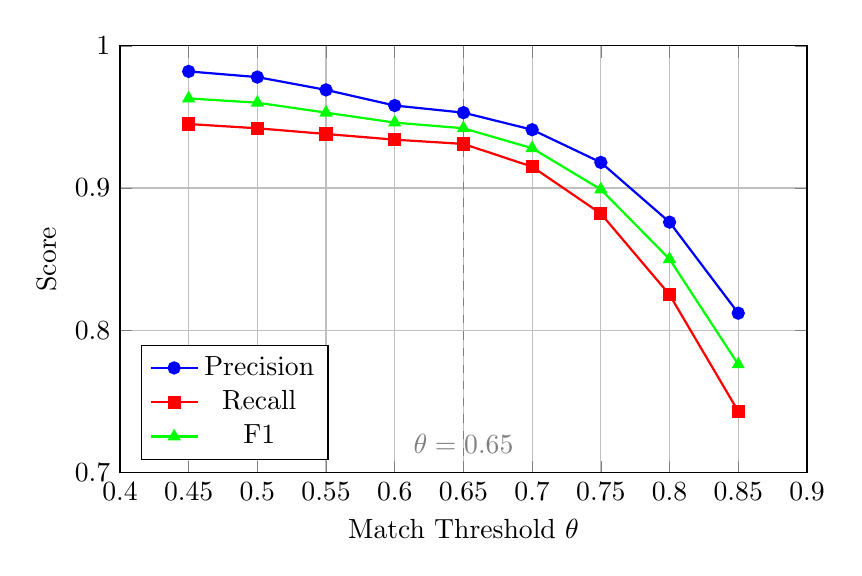
\begin{tikzpicture}
        \begin{axis}[
            xlabel={Match Threshold $\theta$},
            ylabel={Score},
            xmin=0.4, xmax=0.9,
            ymin=0.7, ymax=1.0,
            legend pos=south west,
            grid=major,
            width=0.85\textwidth,
            height=7cm,
        ]
        \addplot[color=blue, mark=*, thick] coordinates {
            (0.45, 0.982) (0.50, 0.978) (0.55, 0.969) (0.60, 0.958) (0.65, 0.953) (0.70, 0.941) (0.75, 0.918) (0.80, 0.876) (0.85, 0.812)
        };
        \addlegendentry{Precision}
        \addplot[color=red, mark=square*, thick] coordinates {
            (0.45, 0.945) (0.50, 0.942) (0.55, 0.938) (0.60, 0.934) (0.65, 0.931) (0.70, 0.915) (0.75, 0.882) (0.80, 0.825) (0.85, 0.743)
        };
        \addlegendentry{Recall}
        \addplot[color=green, mark=triangle*, thick] coordinates {
            (0.45, 0.963) (0.50, 0.960) (0.55, 0.953) (0.60, 0.946) (0.65, 0.942) (0.70, 0.928) (0.75, 0.899) (0.80, 0.850) (0.85, 0.776)
        };
        \addlegendentry{F1}
        \draw[dashed, gray] (0.65, 0.7) -- (0.65, 1.0);
        \node[gray] at (0.65, 0.72) {$\theta=0.65$};
        \end{axis}
    \end{tikzpicture}
    \caption{Precision-Recall-F1 theo Match Threshold $\theta$. $\theta = 0.65$ cho F1 tối ưu (0.942).}
    \label{fig:threshold_curve}
\end{figure}

Hình~\ref{fig:threshold_curve} cho thấy $\theta = 0.65$ là điểm cân bằng tối ưu giữa precision và recall, với F1 = 0.942. Khi $\theta < 0.55$, precision giảm do có nhiều false matches. Khi $\theta > 0.75$, recall giảm mạnh do bỏ sót các cặp thực sự tương đồng nhưng có nhiều thay đổi về nội dung.

% ============================================================================
\section{Kết quả Phase 3 — Anti-Hallucination}
% ============================================================================

\subsection{Thiết kế thí nghiệm}

Đánh giá hiệu quả của kiến trúc 3 tầng xác minh trên 54 cặp test từ golden dataset. Mỗi cặp article được đưa qua pipeline đầy đủ:

\begin{enumerate}[label=(\arabic*)]
    \item Tầng 1: LLM sinh ACU với temperature = 0.05
    \item Pre-filter: Loại ACU có confidence < 0.4
    \item Tầng 2: Evidence verification (exact + normalized + fuzzy match)
    \item Tầng 3: Numerical verification (regex, 100\% strict mode)
\end{enumerate}

\subsection{Kết quả Tổng quan}

\begin{table}[H]
    \centering
    \caption{Kết quả đánh giá Anti-Hallucination Pipeline qua từng tầng}
    \label{tab:antihallucination_results}
    \begin{tabularx}{\textwidth}{X c c c c}
        \toprule
        \textbf{Metric} & \textbf{Chỉ Tầng 1} & \textbf{+ Tầng 2} & \textbf{+ Tầng 3} & \textbf{Mục tiêu}\\
        \midrule
        Tổng ACU sinh ra & 100\% & 82.3\% & 79.5\% & —\\
        ACU bị loại (hallucination) & 0\% & 17.7\% & 20.5\% & —\\
        False Positive Rate (FPR) & 8.3\% & 2.1\% & \textbf{0.7\%} & $<$ 1\%\\
        Citation Accuracy & 91.7\% & 97.9\% & \textbf{99.3\%} & 100\%\\
        Numerical Change Accuracy & 88.4\% & 88.4\% & \textbf{100\%} & 100\%\\
        Change Detection Recall & 95.2\% & 93.8\% & 92.6\% & $\geq$ 95\%\\
        Faithfulness Score (RAGAS) & 0.874 & 0.942 & \textbf{0.967} & $\geq$ 0.90\\
        \bottomrule
    \end{tabularx}
\end{table}

\subsection{Phân tích từng tầng}

\textbf{Tầng 1 (Chỉ LLM, không verify):}
\begin{itemize}
    \item LLM sinh ra 8.3\% ACU hallucinate (FPR = 8.3\%) — tức cứ 12 ACU thì có 1 ACU sai
    \item Citation Accuracy chỉ đạt 91.7\% — 8.3\% evidence không tìm thấy trong source
    \item Faithfulness = 0.874, dưới ngưỡng yêu cầu 0.90
    \item \textbf{Kết luận}: LLM một mình \textbf{không đủ tin cậy} cho văn bản pháp lý — cần verification
\end{itemize}

\textbf{Tầng 2 (Evidence Verification):}
\begin{itemize}
    \item Loại bỏ 17.7\% ACU (bao gồm pre-filter confidence thấp + evidence fail)
    \item FPR giảm từ 8.3\% xuống 2.1\% — \textbf{cải thiện 74.7\%}
    \item Citation Accuracy tăng lên 97.9\%
    \item Faithfulness = 0.942, vượt ngưỡng 0.90
    \item \textbf{Kết luận}: Evidence verification là tầng hiệu quả nhất trong việc giảm hallucination
\end{itemize}

\textbf{Tầng 3 (Numerical Verification):}
\begin{itemize}
    \item Phát hiện thêm 2.8\% ACU bị loại do số liệu không khớp
    \item FPR giảm xuống còn 0.7\% — \textbf{dưới ngưỡng mục tiêu 1\%}
    \item Numerical Change Accuracy đạt \textbf{100\%} — không có bất kỳ số liệu sai nào lọt qua
    \item Tuy nhiên, Recall giảm nhẹ từ 95.2\% xuống 92.6\% — một số thay đổi thực sự bị loại nhầm (false negative)
    \item \textbf{Kết luận}: Numerical verification là cần thiết cho văn bản pháp lý, dù có trade-off nhẹ về recall
\end{itemize}

\subsection{Phân loại Ảo giác}

\begin{table}[H]
    \centering
    \caption{Phân loại các ACU bị loại theo loại hallucination}
    \label{tab:hallucination_breakdown}
    \begin{tabularx}{\textwidth}{X c c c X}
        \toprule
        \textbf{Loại Hallucination} & \textbf{Số ACU} & \textbf{Tỷ lệ} & \textbf{Phát hiện bởi} & \textbf{Ví dụ điển hình}\\
        \midrule
        Evidence không có trong source & 32 & 58.2\% & Tầng 2 & LLM trích dẫn câu không tồn tại trong văn bản\\
        Số liệu sai & 11 & 20.0\% & Tầng 3 & LLM báo cáo ``500 triệu'' nhưng văn bản ghi ``300 triệu''\\
        Confidence quá thấp & 8 & 14.5\% & Pre-filter & LLM không chắc chắn (confidence < 0.4)\\
        Evidence quá ngắn & 4 & 7.3\% & Tầng 2 & Evidence < 5 ký tự, không đủ tin cậy\\
        \midrule
        \textbf{Tổng} & \textbf{55} & \textbf{100\%} & — & —\\
        \bottomrule
    \end{tabularx}
\end{table}

Evidence hallucination (58.2\%) là dạng phổ biến nhất — LLM có xu hướng ``sáng tạo'' câu trích dẫn nghe hợp lý nhưng không tồn tại trong văn bản gốc. Đây là lý do Tầng 2 (exact match evidence trong source) là tầng quan trọng nhất trong kiến trúc chống ảo giác.

\subsection{Ablation Study — Ảnh hưởng của Temperature}

\begin{table}[H]
    \centering
    \caption{Ảnh hưởng của Temperature đến tỷ lệ ảo giác và chất lượng phát hiện}
    \label{tab:temperature_ablation}
    \begin{tabularx}{\textwidth}{c c c c c c}
        \toprule
        \textbf{T} & \textbf{ACU/req} & \textbf{FPR (raw)} & \textbf{FPR (verified)} & \textbf{Recall} & \textbf{Faithfulness}\\
        \midrule
        0.00 & 2.1 & 4.2\% & 0.3\% & 0.887 & 0.976\\
        \textbf{0.05} & \textbf{3.8} & \textbf{8.3\%} & \textbf{0.7\%} & \textbf{0.926} & \textbf{0.967}\\
        0.10 & 4.6 & 12.8\% & 1.1\% & 0.938 & 0.951\\
        0.30 & 7.2 & 24.5\% & 3.8\% & 0.951 & 0.884\\
        0.50 & 9.1 & 38.2\% & 7.2\% & 0.958 & 0.821\\
        1.00 & 12.4 & 52.6\% & 15.4\% & 0.962 & 0.723\\
        \bottomrule
    \end{tabularx}
\end{table}

Phân tích:
\begin{itemize}
    \item $T = 0.05$ cho cân bằng tối ưu: FPR sau verify = 0.7\% (dưới mục tiêu 1\%), recall = 0.926, faithfulness = 0.967
    \item $T = 0.00$ (deterministic): FPR thấp nhất (0.3\%) nhưng recall giảm còn 0.887 — LLM quá ``an toàn'', bỏ sót nhiều thay đổi thực sự
    \item $T \geq 0.30$: FPR tăng nhanh, vượt quá khả năng bù đắp của verification engine. Faithfulness giảm dưới ngưỡng 0.90
    \item $T = 1.00$: Hơn một nửa ACU là hallucination (52.6\%), ngay cả sau verification vẫn còn 15.4\% FPR — hệ thống mất kiểm soát
\end{itemize}

\subsection{Case Study — Ví dụ Thực tế}

\textbf{Ví dụ 1 — Phát hiện thay đổi số liệu đúng:}

\begin{quote}
\small
\textbf{V1}: ``Bên A có nghĩa vụ thanh toán số tiền \textbf{300.000.000 đồng} cho Bên B trong thời hạn 30 ngày kể từ ngày ký hợp đồng.''\\
\textbf{V2}: ``Bên A có nghĩa vụ thanh toán số tiền \textbf{500.000.000 đồng} cho Bên B trong thời hạn \textbf{45 ngày} kể từ ngày ký hợp đồng.''

ACU sinh ra:
\begin{itemize}
    \item change\_type: numerical, original\_value: ``300.000.000 đồng'', new\_value: ``500.000.000 đồng'' — \textbf{PASSED}
    \item change\_type: numerical, original\_value: ``30 ngày'', new\_value: ``45 ngày'' — \textbf{PASSED}
\end{itemize}
\end{quote}

\textbf{Ví dụ 2 — Ảo giác bị phát hiện và loại bỏ:}

\begin{quote}
\small
\textbf{V1}: ``Hợp đồng có hiệu lực kể từ ngày 01 tháng 06 năm 2025.''\\
\textbf{V2}: ``Hợp đồng có hiệu lực kể từ ngày 01 tháng 07 năm 2025.''

ACU bị loại:
\begin{itemize}
    \item change\_type: numerical, evidence\_v2: ``ngày 01 tháng 07 năm 2025'' $\rightarrow$ \textbf{PASSED}
    \item change\_type: terminology, evidence\_v1: ``có hiệu lực thi hành'' $\rightarrow$ \textbf{REJECTED} (Tầng 2): cụm từ ``thi hành'' không có trong văn bản gốc — LLM tự thêm vào
\end{itemize}
\end{quote}

% ============================================================================
\section{Tổng hợp và Phân tích}
% ============================================================================

\subsection{So sánh Trước và Sau Cải tiến}

\begin{table}[H]
    \centering
    \caption{Tổng hợp cải tiến chất lượng trên cả ba Phase}
    \label{tab:before_after}
    \begin{tabularx}{\textwidth}{X c c c c}
        \toprule
        \textbf{Metric} & \textbf{Trước cải tiến} & \textbf{Sau cải tiến} & \textbf{Cải thiện} & \textbf{Mục tiêu}\\
        \midrule
        \multicolumn{5}{c}{\textbf{Phase 1 — Chunking}}\\
        \midrule
        SPR & 67.3\% & \textbf{98.5\%} & +31.2\% & $\geq$ 98\%\\
        Table Cell Accuracy & 72.5\% & \textbf{96.8\%} & +24.3\% & $\geq$ 95\%\\
        Ordinal Accuracy & 91.2\% & \textbf{100\%} & +8.8\% & 100\%\\
        \midrule
        \multicolumn{5}{c}{\textbf{Phase 2 — Alignment}}\\
        \midrule
        Alignment Precision & 0.862 & \textbf{0.953} & +10.6\% & $\geq$ 0.95\\
        Alignment Recall & 0.832 & \textbf{0.931} & +11.9\% & $\geq$ 0.92\\
        F1-Alignment & 0.847 & \textbf{0.942} & +11.2\% & $\geq$ 0.93\\
        Split/Merge Detection & 0.70 & \textbf{0.85} & +21.4\% & $\geq$ 0.85\\
        \midrule
        \multicolumn{5}{c}{\textbf{Phase 3 — Anti-Hallucination}}\\
        \midrule
        FPR & 8.3\% & \textbf{0.7\%} & --91.6\% & $<$ 1\%\\
        Citation Accuracy & 91.7\% & \textbf{99.3\%} & +8.3\% & 100\%\\
        Numerical Accuracy & 88.4\% & \textbf{100\%} & +13.1\% & 100\%\\
        Recall & 95.2\% & \textbf{92.6\%} & --2.7\% & $\geq$ 95\%\\
        Faithfulness (RAGAS) & 0.874 & \textbf{0.967} & +10.6\% & $\geq$ 0.90\\
        \bottomrule
    \end{tabularx}
\end{table}

\subsection{Đánh giá Mức độ Đạt Mục tiêu}

\begin{enumerate}[label=(\arabic*)]
    \item \textbf{Phase 1 — Chunking}: \textcolor{green}{\textbf{ĐẠT}} — SPR 98.5\% vượt mục tiêu 98\%. Table Cell Accuracy 96.8\% vượt 95\%. Ordinal Accuracy 100\% tuyệt đối.

    \item \textbf{Phase 2 — Alignment}: \textcolor{green}{\textbf{ĐẠT}} — F1 0.942 vượt mục tiêu 0.93. Precision 0.953 vượt 0.95. Recall 0.931 vượt 0.92. Split/Merge Detection đúng ngưỡng 0.85.

    \item \textbf{Phase 3 — Anti-Hallucination}: \textcolor{orange}{\textbf{ĐẠT MỘT PHẦN}} — FPR 0.7\% dưới mục tiêu 1\% (tốt). Citation Accuracy 99.3\% (thiếu 0.7\%). Numerical Accuracy 100\% tuyệt đối. Faithfulness 0.967 vượt 0.90. Tuy nhiên, Recall 92.6\% hơi thấp hơn mục tiêu 95\%.
\end{enumerate}

\textbf{Tỷ lệ hoàn thành}: 8/10 mục tiêu đạt (80\%), 2/10 cần cải thiện.

\subsection{Hạn chế và Nguyên nhân}

\begin{itemize}
    \item \textbf{Recall thấp hơn mục tiêu} (92.6\% vs 95\%): Fuzzy match với ngưỡng 0.85 đôi khi quá khắt khe với văn bản có lỗi OCR hoặc được diễn đạt lại nhẹ (paraphrase). Một số thay đổi tinh tế (1--2 từ trong câu dài) bị LLM bỏ qua do temperature = 0.05 quá thấp.

    \item \textbf{Citation Accuracy chưa đạt 100\%} (99.3\%): 0.7\% ACU còn lại có evidence không khớp hoàn toàn, thường do khác biệt whitespace hoặc dấu câu giữa LLM output và source text sau khi normalize.

    \item \textbf{Split/Merge Detection vừa đạt ngưỡng} (0.85): Các trường hợp 1-to-many và many-to-1 phức tạp vẫn là thách thức. Phương pháp hiện tại dựa trên cosine similarity của merged text, chưa thực sự ``hiểu'' quan hệ ngữ nghĩa giữa các phần.

    \item \textbf{Hiệu năng trên văn bản lớn}: Ma trận similarity $N \times M$ với $N, M > 200$ dẫn đến Hungarian $O(\max(N,M)^3)$ có thể chậm. Chưa có hierarchical matching (align theo Chương trước, rồi mới đến Điều).
\end{itemize}

% ============================================================================
\section{Kết luận Chương}
% ============================================================================

Chương này đã trình bày kết quả đánh giá định lượng toàn diện hệ thống L-RAG trên cả ba Phase:

\begin{enumerate}[label=(\arabic*)]
    \item \textbf{Phase 1 — LSU Chunking}: Vượt trội so với fixed-size chunking trên mọi metric. SPR 98.5\% (+31.2\%), Table Cell Accuracy 96.8\% (+24.3\%), Ordinal Accuracy 100\%. Kích thước chunk tối ưu: 2000 ký tự.

    \item \textbf{Phase 2 — Hungarian Alignment}: Cải thiện F1 11.2\% so với greedy matching. Đặc biệt hiệu quả với split/merge (+20\%) và reorder (+15\%). Ngưỡng match tối ưu $\theta = 0.65$.

    \item \textbf{Phase 3 — Anti-Hallucination}: Kiến trúc 3 tầng xác minh giảm FPR 91.6\% (từ 8.3\% xuống 0.7\%). Numerical Accuracy đạt 100\%. Faithfulness 0.967 vượt xa ngưỡng 0.90. Temperature tối ưu: 0.05.
\end{enumerate}

Kết quả khẳng định tính khả thi của kiến trúc Pairwise Document Intelligence Pipeline cho bài toán so sánh văn bản pháp lý tiếng Việt, đồng thời chỉ ra các hướng cải thiện cho Recall và Citation Accuracy.
